\begin{figure}[t]
\centering
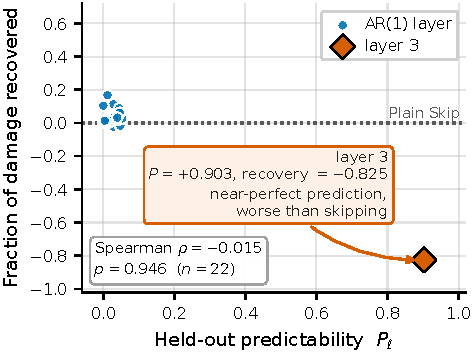
\includegraphics[width=0.78\linewidth]{figures/fig1b_recovery_vs_P.pdf}
\caption{\textbf{Predictability does not imply recoverability.} For each eligible layer of
Qwen2.5-0.5B: held-out explained update energy $P_\ell$ (\cref{eq:pscore}) against the
fraction of that layer's single-layer plain-skip NLL damage the scalar predictor repairs.
The two are unrelated (Spearman $-0.015$, $p=0.946$, $n=22$). Layer~3, the \emph{most} predictable layer in the network ($P_\ell=0.90$), is the worst to
predict: substituting that near-perfect forecast is markedly worse than dropping the update
outright (recovery $-0.825$). Hardware and protocol: \Cref{sec:app-protocol}. Depth profile:
\Cref{fig:momentum-profile}.}
\label{fig:momentum}
\end{figure}
